\chapter{Response to the referees}
I would like to thank all three referees for their valuable insights and help to refine the dissertation. Please be sure I carefully addressed all your comments, even those I have decided not to integrate into the final version fully.

\section{Doc. PhDr. Adam Ger\v{s}l Ph.D.}

\textbf{\textit{Comments to the first paper on ``What Type of Finance Matters for Growth? Bayesian Model Averaging Evidence''}}

% {\itshape The dissertation thesis is a collection of three very well written empirical papers exploring the links between financial development on one hand and long-term economic growth, wealth inequality, and income inequality on the other hand. The author demonstrates strong skills in using up-to-date econometric methods, especially the Bayesian Model Averaging (BMA), to analyze available data on relevant economic phenomena. The first paper titled ``What Type of Finance Matters for Growth? Bayesian Model Averaging Evidence'' explores the finance-growth link with an updated dataset on long-term per capita GDP growth, a number of economic and institutional factors, and selected variables capturing financial intermediation. The value added is in using the BMA framework to account for model uncertainty and in testing the explanatory power of five selected financial development indicators: in addition to the traditional credit to GDP and stock market capitalization (both capturing the depth of financial intermediation), the paper uses a measure of bank efficiency (net interest margin), a measure of stock market activity (turnover rate), and a measure of bank stability (the Z-score). The author finds that especially the bank efficiency measure is robustly related to long-term economic growth, which much higher inclusion probability than the traditional financial depth indicators.

% The second paper on ``Finance and Wealth Inequality'' uses the BMA framework to explore the link between financial, economic and institutional factors and the wealth Gini coefficient for a sample of 73 countries. The results show that finance has a multi-faced impact on wealth inequality – financial depth increases inequality, but efficiency and access to finance decrease it.

% The final paper investigates the link between financial intermediation and income inequality within a panel BMA framework. Also this paper finds that finance has a complex impact on inequality – the access to finance and efficiency decrease it, while the size of markets does not have any significant impact.

% There is an original contribution of the author in all three essays, all are based on relevant references, and all would be in my view defendable as a part of dissertation at respected universities. They are all written in a clear language and definitely publishable (actually, the first one has been published already in the World Bank Economic Review and the second in the Journal of International Money and Finance). While the focus is on data analysis and deriving relationships based on regression techniques, the thesis would benefit from a few revisions that would emphasize economic understanding, especially when interpreting the findings of the statistical exercises.

% My general assessment is that the thesis can be defended after revision indicated in my comments below.}

\begin{enumerate}
       
    \item \textit{The title is confusing - the paper does not explore what type of finance (bank versus market; bond versus stocks; banks versus non-bank institutions; short-term versus long-term; concentrated versus unconcentrated banking sector etc.) matters for growth, but what aspect of financial intermediation (financial depth; activity on markets; efficiency of banks; resilience of banks) matter. I propose to adjust the title accordingly.}
    
    Thank you for the valid point and a suggestion of an alternative. I changed the title of the first paper to \emph{What Aspect of Financial Intermediation Matters for Growth: Bayesian Model Averaging Evidence}. I adjusted the footnote referring to the chapter's publication so that it reflects the title of the published paper.

    \item \textit{The endogeneity problem (briefly mentioned on p. 11) is much more serious than the author thinks as the variables get averaged over 50 years! The studies focusing on the dynamics of development between the real and financial sector (macrofinancial linkages, such as in Crowe et al. 2010) emphasize the two-way interactions and feedbacks that develop over time. As the methodology does not take into account the time dynamics, the thesis should at least acknowledge that endogeneity could be an issue and devote a paragraph or so to this shortcoming, adding a few references on the (omitted) dynamic interactions.}
    
    The point is well taken. Although the issue of endogeneity gets mentioned throughout the paper, it might come out as underappreciated. I have explicitly added a subsection discussing potential endogeneity and the limitations of our attempts to address it. While we can efficiently deal with the potential omitted variable bias by applying \ac{BMA}, the risk lies mainly in the reverse causality. To estimate where we use the lagged financial indicators and look at the shorter growth period, I added the results on the two-stage least squares \ac{BMA} that previously appeared in one of the footnotes and available upon request. Since finding the right instruments for our financial variables is a challenge, we focused this robustness exercise on the net interest margin to measure financial intermediation efficiency. Using the history of financial crises as an instrumental variable, we obtain results that support the baseline finding that intermediation efficiency is conducive to long-run growth.
    
    \item \textit{Throughout the paper, the net interest margin (NIM) is interpreted as a measure of ``efficiency of financial intermediaries'', but this is incorrect! It is a measure of (in)efficiencies in financial intermediation, not an indicator of bank (cost) efficiency! Large NIMs are typical for underdeveloped markets in which risks (of default), vulnerabilities, and legal uncertainties (of collateral realization etc.) are large, increasing information asymmetries and creating frictions to (efficient) financial intermediation. Thus, the NIM is actually an additional (indirect) measure of the institutional (legal) framework within which financial intermediation takes place rather than ``an aspect'' of financial activity.}

    Thank you for elaborating on this issue. I have partially adjusted the wording throughout the first paper and I have added an introductory part in the summary of the dissertation about different approaches to the 'efficiency' in finance and how we understand it to be able to use efficiency of financial intermediaries interchangeably with the efficiency of financial intermediation. % This also reflects one of the comments by Mr. \v{C}ih\'{a}k.

    \item \textit{Given the previous point, the author should be much more careful in drawing conclusions from the analysis. The fact that his measure of efficiency has a large PIP might be to a large extent related to the endogeneity bias: as an economy develops, the overall risks and vulnerabilities decline, contributing to a decline of the margin, which goes hand in hand with expansion in lending, further supporting economic development. This link should be mentioned in the paper.}    
    
    I partly address this comment in one of the related above. I have extended the section devoted to discussing endogeneity. Although in a crude way, I tackle it in robustness check with lagged values of financial indicators similar to the approach in the second paper on finance and wealth. The time span is shorter (10 years) and admittedly involves the aftermath of the financial crisis, but nevertheless, the conclusions are consistent with the baseline, and it limits the mentioned risks to some extent. I agree that by averaging variables over long time spans, we lose information on the short-run dynamics, and net interest margin may potentially mask the effect of another variable. We attempt to avoid that by accounting for a large volume of potential institutional factors explicitly in \ac{BMA} (rule of law, political rights, degree of capitalism, or openness of economy). In the 2SLS--BMA estimation, we include these potentially confounding factors in the first-stage regression.

    \item \textit{The review of literature mentions the criticism of traditional finance-growth nexus papers in neglecting the private bond markets (and other non-bank or non--stock--market sources of finance), but the paper again uses only the two traditional measures of financial depth -- bank credit and stock market (p. 10). Could the private credit to GDP be based on the BIS statistics of total credit (i.e. a sum of bank credit, non-bank intermediaries credit, bonds issues, and cross-border finance to private sector)? This has become available recently for a large number of countries (and years) and could better capture the debt of the private sector intermediated by all intermediaries and markets.}
    
    Thank you for pointing me to the \ac{BIS} data. Unfortunately, the coverage is insufficient to allow for using the data as-is. Simply merging the data with our dataset reduces the number of observations to 33 and renders the baseline approach infeasible. Nevertheless, for the available data point, the correlation between total credit and bank credit data reaches nearly 0.7 (see also Figure \ref{app:total_bank_credit}). I have thus re-estimated the model with partially modified total credit data from \ac{BIS}. I used the bank credit to non-financial sector data from \ac{GFDD} to estimate the total credit volumes for the countries with missing data. Next, I applied the \ac{BMA} using total credit instead of bank credit (and dropping the later from the set of covariates). Total credit shows low \ac{PIP}, and none of the other relevant regressors is affected. Using the fitted values of total credit for all observations instead of only the missing values does not alter the results in any way. In Table \ref{chA:tab1}, I only report \acp{PIP} along with the moments of the top covariates and total credit.

\end{enumerate}

\begin{figure}[ht!]
  \caption{Total vs. bank credit to non-financial sector}
  \label{app:total_bank_credit}
  \centering
  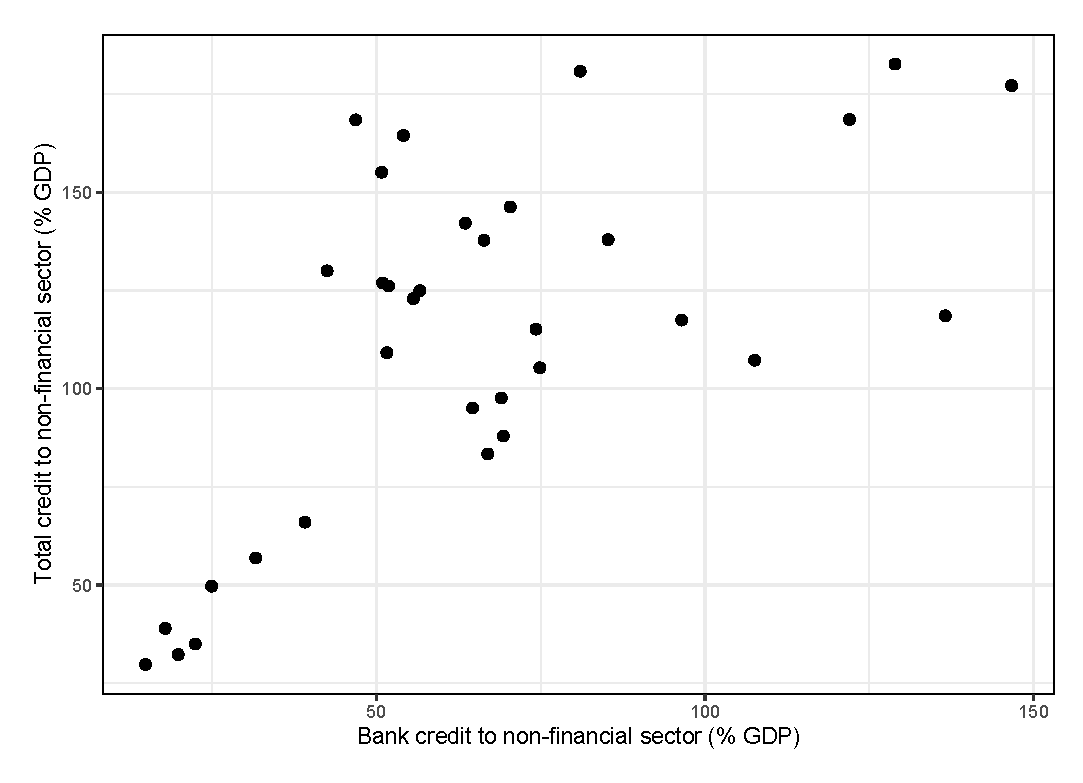
\includegraphics[width=0.8\textwidth, keepaspectratio]{figures/app/totalcredit_bankcredit}
\end{figure}

\begin{table}[ht!]
  \caption{Results total credit to non-financial institutions.}\label{chA:tab1}
    \footnotesize
    \centering
  \begin{tabular}{lrrr}
    \toprule
                                 & PIP & Post Mean & Post SD \\
    \midrule
    GDP level in 1960 & 1.00 & -0.01075 & 0.00241 \\
    Fraction GDP in mining & 1.00 & 0.04705 & 0.01344 \\
    Exchange rate distortions & 1.00 & -0.00009 & 0.00003 \\ 
    Fraction Confucian & 1.00 & 0.03898 & 0.01117 \\
    Life expectancy & 1.00 & 0.00058 & 0.00020 \\
    Fraction Buddhist & 0.99 & 0.01265 & 0.00495 \\ 
    Net interest margin & 0.96 & -0.00114 & 0.00047 \\ 
    Equipment investment & 0.83 & 0.07263 & 0.04768 \\
    \vdots \\
    \textbf{Total private credit} & 0.04 & 8.6345e-08 & 0.00001 \\
    \vdots \\
    \bottomrule
  \end{tabular}
\end{table}

\clearpage
\noindent \textbf{\textit{Comments to the second paper on ``Finance and Wealth Inequality''}}

\begin{enumerate}[resume]

    \item \textit{In comparison to the previous paper, this one tackles well a possible endogeneity bias (section 3.5.3) by lagging the explanatory variables (average of 1980-2009) compared to the dependent variable (average of 2010-2016), although I would be less concerned about the reverse link between inequality and financial development (compared to GDP growth and financial development). While a paragraph explaining through which channels would wealth inequality influence financial development is included on p. 66 (with reference to Beck et al. 2007), I am not too persuaded by (the two) explanations. Could 1-2 additional references be provided if, as the author states, ``the question of endogeneity is deeply ingrained in the finance-inequality nexus''? (Some additional arguments are included in the third paper and could be re-used here).}
    
    The firm wording is due to the universally present concerns about endogeneity in the finance-inequality literature\footnote{To name a few: \textcite{cihaksahay2020,de2017finance,goda2017income,bazillier2017circular,kumhof2015inequality,mookerjee2010availability}}. I have included additional references on the issue in the endogeneity section of the paper, including the previously omitted inequality and financial crises branch of studies.
        
    \item \textit{In this paper, an overall index of efficiency is used, combining the net interest margin with variables such as overhead costs or profitability. I would still propose that this index is not called Financial Institutions Efficiency (but perhaps Financial Intermediation Efficiency) because it combines institutions' (cost) efficiency and efficiency (frictions) of financial intermediation influenced by overall risks. As this indicator has a 100\% PIP, it would be worth exploring further what drives the efficiency index -- is it more the NIM/spread as a measure of inefficiencies in financial intermediation (risks) or (overhead) costs as a measure of financial institutions' efficiency?}
    
    I took two different approaches to explore the details of the FIE measure. First, the methodological paper to the financial development data by the IMF \parencite{svirydzenka2016introducing} provides the weights applied to the observed series to construct the indicator of financial intermediation efficiency. These are the loading factors in the principal component analysis, which capture the common variation in the data related to the same category. This approach helps to correct for the overlapping information among multiple efficiency indicators and provides the basis for their aggregation. In the case of FIE, the largest weight is on the overhead costs (25\%), net interest margin (20\%), lending-deposit spread, and non-interest income (both roughly 17\%). ROA and ROE both enter with relatively lower weights slightly above 10\%.

    The second approach relies on \ac{BMA} estimation with the underlying series of the FIE. I mirror the baseline methodological procedure using the individual indicators and report the results in Table \ref{chA:tab2}. The most important characteristics, according to the \ac{PIP} are the overhead costs and net interest margin, both attaining values above 0.5. Both variables exhibit the expected positive posterior mean. The higher net interest margin and overhead costs associate with higher levels of wealth inequality as measured by Gini index. Unfortunately, I had to drop lending-deposit spread since the data was missing on the part of the observations. The remaining components of intermediation efficiency show low inclusion probabilities.

    The IMF's procedure and the estimate presented here thus show consistent results putting net interest margin and overhead costs upfront in capturing intermediation efficiency and its accompanying effects. Somewhat lower \acp{PIP} relative to the combined efficiency measure may arise from the collinearity between the individual indicators.
    
    \begin{table}[ht!]    
      \caption{Results using the individual components of financial intermediaries' efficiency}\label{chA:tab2}
      \centering
      \footnotesize
      \begin{tabular}{lrrr}
        \toprule
      Variable & PIP & Post Mean & Post SD \\
        \midrule
      Value added in agriculture & 1.00 & -0.53450 & 0.17265 \\
        Access to financial institutions & 0.99 & -0.38380 & 0.16285 \\ 
        Number of war years & 0.95 & 0.19154 & 0.10297 \\ 
        Outward orientation & 0.69 & 0.12387 & 0.11848 \\
        Economic freedom index (adjusted) & 0.66 & -0.22199 & 0.22503 \\ 
        Financial market depth & 0.60 & 0.25546 & 0.25381 \\
        \textbf{Net interest margin} & 0.57 & 0.22508 & 0.25392 \\ 
        \textbf{Overhead costs / Assets} & 0.56 & 0.16033 & 0.18376 \\ 
        Business conditions & 0.55 & -0.11950 & 0.14897 \\
        Financial institutions depth & 0.52 & 0.29136 & 0.33501 \\ 
        Inflation & 0.52 & 0.08456 & 0.10874 \\ 
        Education index (UN) & 0.51 & -0.15375 & 0.20071 \\
        Redistribution & 0.45 & -0.09356 & 0.13734 \\ 
        Net national savings & 0.30 & 0.04713 & 0.09898 \\
        Natural resources rents & 0.28 & 0.04244 & 0.09185 \\ 
        Labour market regulation & 0.26 & 0.03507 & 0.08022 \\
        Pre-tax ROA & 0.24 & -0.04709 & 0.12282 \\ 
        Net foreign direct investment & 0.23 & -0.02525 & 0.06581 \\
        Latin America dummy & 0.20 & 0.06632 & 0.20283 \\
        Financial openness (Chinn-Ito) & 0.14 & 0.01615 & 0.06855 \\
        Population density & 0.14 & -0.01313 & 0.05141 \\ 
        Rule of law & 0.13 & 0.02374 & 0.10437 \\
        Leftwing orientation & 0.12 & -0.00996 & 0.04222 \\ 
        Pre-tax ROE & 0.12 & 0.01714 & 0.07991 \\
        Banking diversification & 0.12 & -0.00837 & 0.03859 \\
        Public education expenditures & 0.12 & 0.00914 & 0.04335 \\ 
        Revolutions and coups & 0.11 & 0.00894 & 0.04639 \\
        Civ. liberties and Pol. rights & 0.10 & -0.01329 & 0.06491 \\
        Financial markets efficiency & 0.10 & 0.00863 & 0.04648 \\
        Financial liberalization (EFW) & 0.08 & 0.00169 & 0.05097 \\ 
        Life expectancy & 0.08 & -0.00032 & 0.06619 \\ 
        GDP level in 1990 & 0.08 & 0.00768 & 0.09478 \\
        Population growth & 0.08 & 0.00413 & 0.04553 \\
        Active banking restrictions & 0.07 & -0.00337 & 0.03223 \\ 
        Average GDP growth & 0.07 & -0.00390 & 0.03385 \\
        Bank capital regulations & 0.07 & -0.00426 & 0.02943 \\
        Non-interest income & 0.07 & 0.00133 & 0.03183 \\
        Technological progress & 0.06 & -0.00170 & 0.06215 \\ 
        Government expenditures & 0.06 & 0.00280 & 0.03468 \\
        Labour force participation & 0.06 & -0.00219 & 0.08291 \\
        Value added in industry & 0.05 & 0.00102 & 0.02998 \\ 
         \bottomrule
      \end{tabular}
      \end{table}

\noindent \textbf{\textit{Comments to the third paper on ``Finance and Inequality --- Panel BMA Approach''}}

    \item \textit{The paper could better formulate what is the value added compared to available literature. There are a few hints in the last paragraph on page 99, but this could be better structured and start with ``The value added of this paper is in \dots''. Using the after-tax rather than before-tax measure of income distribution should also be mentioned here (and explained why).}
    
    Thank you for pointing this out. I have included a paragraph on the value-added of the paper. I make four different points. First, we efficiently account for model uncertainty relying on the panel \ac{BMA} framework. Second, we use the \ac{WID} data on the top income shares, collected based on the tax collection data. Arguably, this data is superior to the survey data as it amends issues of underrepresentation of high-income individuals and underreporting income. Third, we simultaneously consider different proxies of financial development to identify the most relevant channels through which finance affects inequality and, fourth, we examine multiple measures of income inequality to distinguish the diverse effects of finance across the income distribution.
    
    
    We rely on the after-tax income Gini coefficient as we also include the redistribution variable among the regressors to indirectly account for taxation and transfers, as coverage of exact data on the two is scarce. Since we define it as a difference between before-tax and after-tax Gini coefficients, the estimate is not substantially influenced by using either of the two as the dependent variable. The switch changes only the sign of the posterior mean of redistribution. This supports the point by \textcite{furceri2019robust} that unless redistribution is systematically correlated with other regressors, their effect on the net and gross inequality should be the same. In our case, using after-tax allows for more intuitive interpretation. In Table \ref{chA:tab3}, I provide the estimation with the before-tax Gini coefficient as the dependent variable. I report only the regressors with \ac{PIP} above 0.7 as the results are nearly identical to the baseline estimate.

\begin{table}[!ht]
  \caption{Results with before-tax income Gini coefficient as dependent variable}\label{chA:tab3}
    \footnotesize
\centering
\begin{tabular}{lrrr}
  \toprule
 & PIP & Post Mean & Post SD \\
  \midrule
  Unemployment & 1.00 & 0.22926 & 0.05717 \\
  Non-equipment investment & 1.00 & 0.14580 & 0.05064 \\
  Access to financial institutions & 1.00 & -0.24226 & 0.06077 \\ 
  Education index (UN) & 1.00 & -0.57258 & 0.23138 \\
  Redistribution & 1.00 & 0.21473 & 0.04871 \\ 
  Education index sq. & 1.00 & 0.80725 & 0.21188 \\
  GDP per capita & 1.00 & 1.62403 & 0.55557 \\ 
  Education expenditures & 1.00 & -0.14092 & 0.04896 \\
  GDP per capita sq. & 1.00 & -1.44382 & 0.56148 \\ 
  Economic freedom & 0.99 & 0.17956 & 0.06767 \\ 
  Life expectancy & 0.98 & -0.22629 & 0.09737 \\
  Value added in agriculture & 0.92 & -0.11102 & 0.06240 \\ 
  Government expenditures & 0.90 & 0.11397 & 0.06028 \\
  Total population & 0.90 & -0.14643 & 0.08616 \\ 
  Financial institutions efficiency & 0.85 & -0.08345 & 0.05623 \\
  Inflation & 0.74 & 0.13437 & 0.12365 \\ 
  \vdots \\
  \bottomrule
\end{tabular}
\end{table}
    
    \item \textit{Averaging the data across 3-year spans to produce the panel (over 2000-2014) is a standard method to get rid of short-term volatility in the data say from markets, but given that this coincides with the largest economic pre-crisis boom 2000-2007 and the crisis and post-crisis decline associated with balance-sheet recessions in many countries (2008/2009-2014), it will not get rid of the business cycle. The more traditional 5-year averaging would be better. As this was done as a robustness check (with similar results), I would propose to use the 5-year averaging as a baseline and the 3-year averaging as a robustness check.}
    
    I understand the preference for 5-year averaging. Nevertheless, I have decided to stay with the 3-year averages. Several reasons support this decision. First, the 3-year models display much better convergence, which I grant to more available observations and the higher variation in the 3-year averaged data. Second, more time periods allow for a more robust estimate when I lag the explanatory variables in order to address endogeneity. Third, I am not convinced that in the case of the concerned period 2000-2014, 5-year averages notably superior in getting rid of the one long business cycle we observed. I expanded the discussion on the choice by preceding arguments and added the 5-year results to the paper's Appendix. I also contrast the estimate under different averages and for alternative inequality measures here in the response (figures \ref{ch4fig:comp_3y5y_gini}, \ref{ch4fig:comp_3y5y_top10}, \ref{ch4fig:comp_3y5y_top1}). The largest differences occur with the Gini index as the dependent variable. Note the large increase of time period dummies in case of 5-year averages. They might mask some of the explicitly captured effects before, e.g., changes in economic freedom index, government expenditures, or inflation. Nothing substantially changes our conclusions about financial indicators. The results for top income share appear to be even more stable, except for volatile \ac{PIP} of inflation.

    \begin{figure}[ht!]
      \caption{Comparison of results between 3-year and 5-year averaged data, after-tax Gini index}
      \label{ch4fig:comp_3y5y_gini}
      \centering
      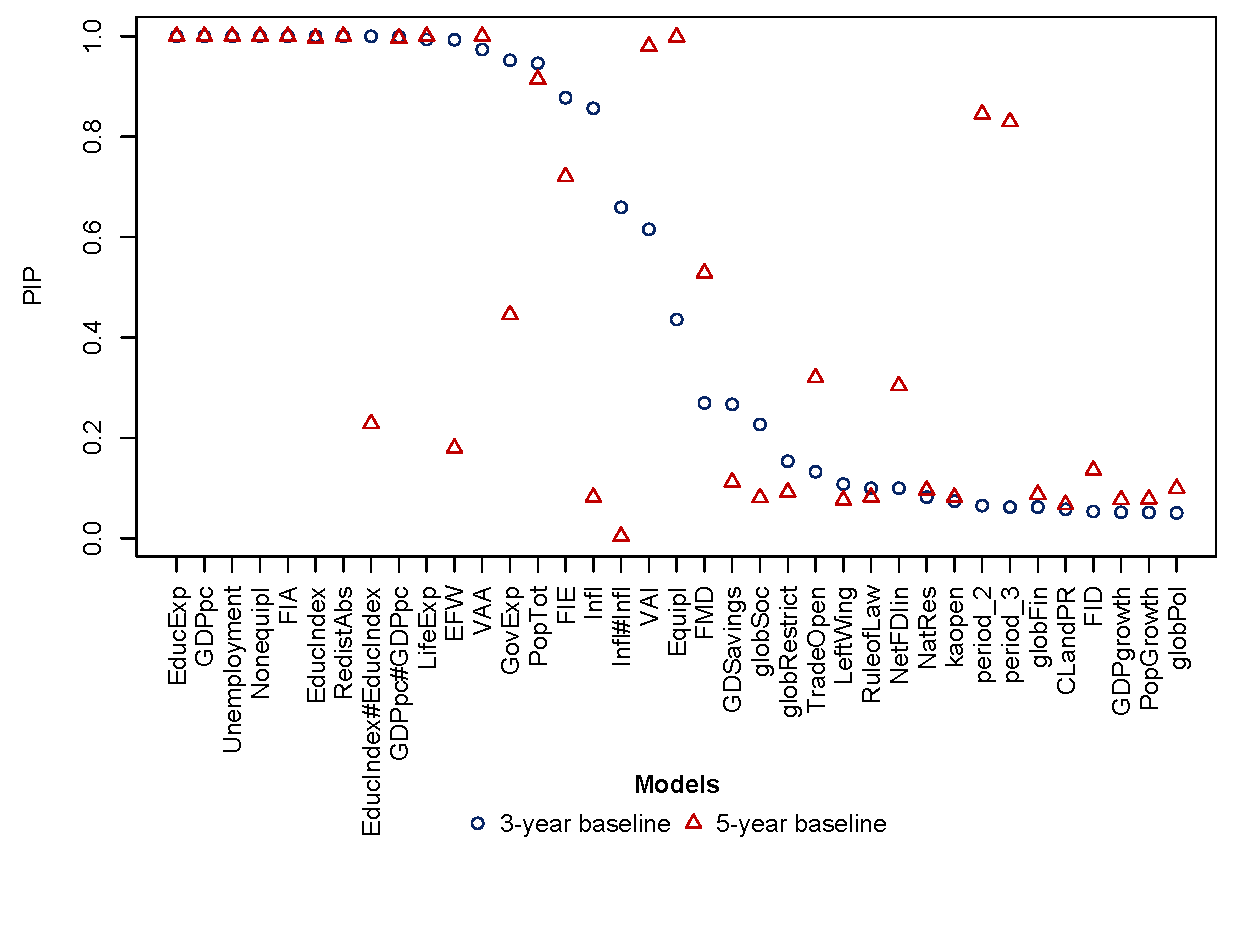
\includegraphics[width=0.8\textwidth, keepaspectratio]{Figures/ch4/comp_3y5y_gini}
      % \begin{minipage}{0.8\textwidth}
        % \footnotesize
        % \emph{Note: The comparison only shows variables which show \ac{PIP} $> 0.9$ in at least one of the models.}
        % \end{minipage}
    \end{figure}
\clearpage
    \begin{figure}[ht!]
      \caption{Comparison of results between 3-year and 5-year averaged data, top 10\% share}
      \label{ch4fig:comp_3y5y_top10}
      \centering
      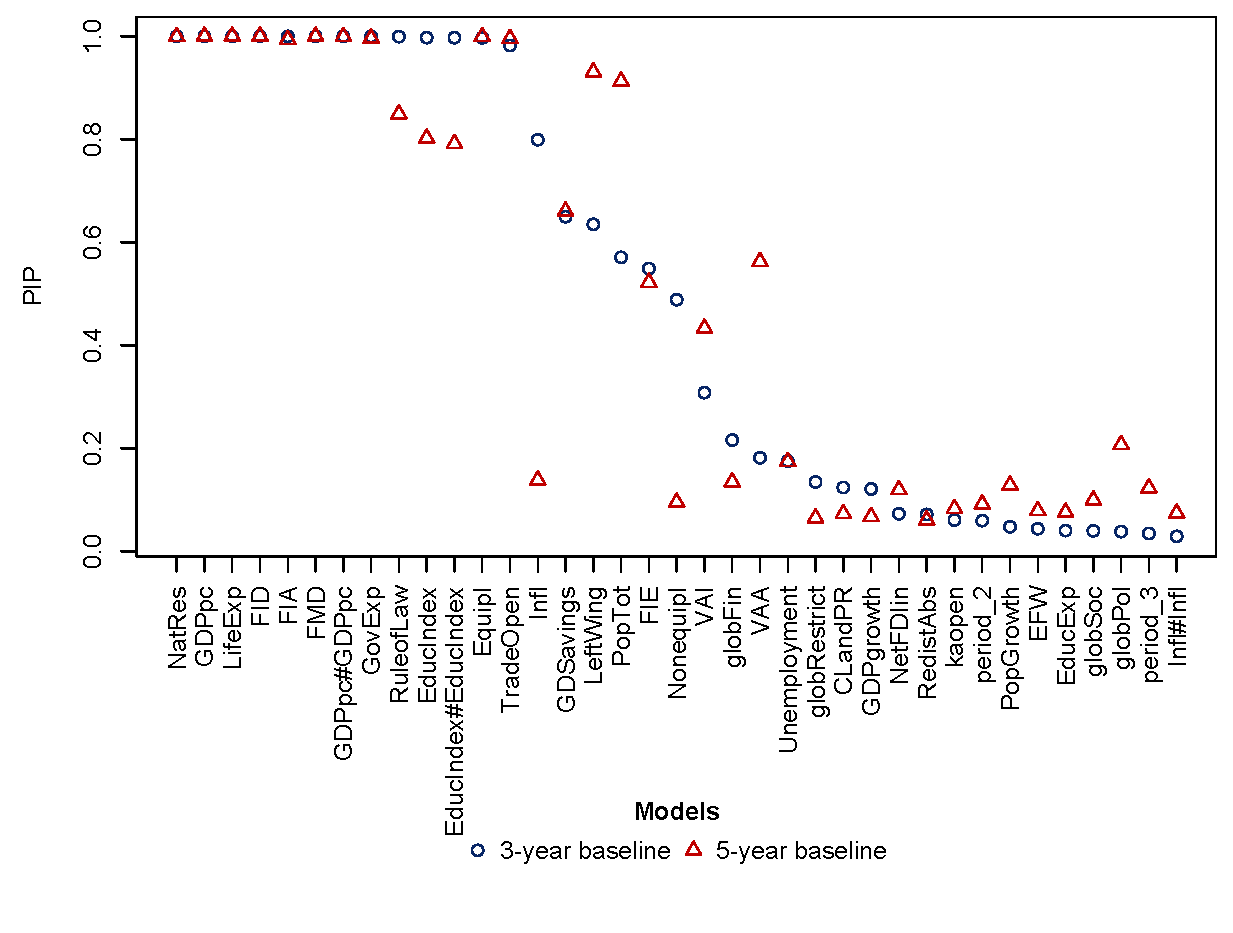
\includegraphics[width=0.8\textwidth, keepaspectratio]{Figures/ch4/comp_3y5y_top10}
      % \begin{minipage}{0.8\textwidth}
        % \footnotesize
        % \emph{Note: The comparison only shows variables which show \ac{PIP} $> 0.9$ in at least one of the models.}
        % \end{minipage}
    \end{figure}

    \begin{figure}[ht!]
      \caption{Comparison of results between 3-year and 5-year averaged data, top 1\% share}
      \label{ch4fig:comp_3y5y_top1}
      \centering
      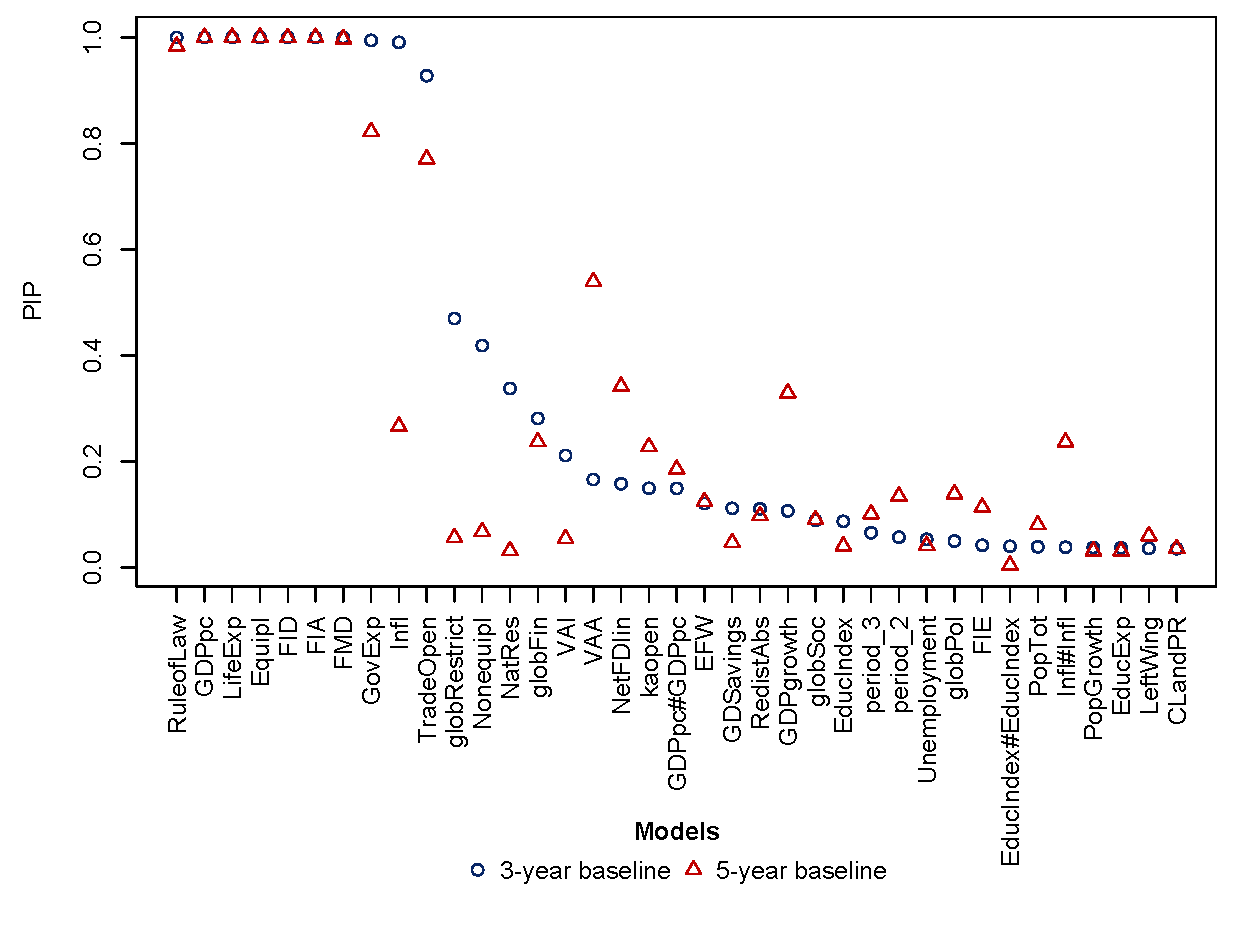
\includegraphics[width=0.8\textwidth, keepaspectratio]{Figures/ch4/comp_3y5y_top1}
      % \begin{minipage}{0.8\textwidth}
        % \footnotesize
        % \emph{Note: The comparison only shows variables which show \ac{PIP} $> 0.9$ in at least one of the models.}
        % \end{minipage}
    \end{figure}
\clearpage
    \item \textit{Another robustness check could be to split the sample into two periods only, pre-crisis 2000-2007 and post-crisis 2008-2014, creating two 7-year averages. Instead of a panel, two cross-sections would be run and results could be interpreted as regime-specific (pre-crisis versus post-crisis regimes).}
    
    Thank you for the suggestion. Relying on the cross-section disregards the time variation of the data and makes the comparison to the baseline estimations difficult. Instead, I have split the sample as you outlined, but kept still relied on fixed effects \ac{BMA}. I present here only the regime comparisons of pre- / post- crisis estimates for all income inequality indicators. There is a lot of variation in terms of inclusion probability under the two alternatives, partially because I a switch to yearly panel data to make the estimation feasible. I focus here only on the interpretation of financial indicators. Access to finance appears robustly across specifications. In comparison with the baseline results, the efficiency of intermediation has very high \ac{PIP} in the post-crisis sample for the overall distribution and top 10\% share. Similarly, FID displays much higher \ac{PIP} after 2007 in the estimation with the Gini index estimation. Both suggest that financial institutions had a mitigating effect on the post-crisis development of inequality. On the other hand, the share of the very top percentile of the income distribution was driven, among other things, by the depth of financial markets and institutions. The fact that the effect of finance on the economy differs across the business cycle is established \parencite{braun2005finance,DellAricciaetal2008} and may manifest further in income inequality. Given the regimes' overall differences, I caution against putting too much weight on these results though.
    
    \begin{figure}[ht!]
      \caption{Pre- / post- 2007 crisis comparison, after-tax Gini index}
      \label{ch4fig:comp_prepostcrisis_gini}
      \centering
      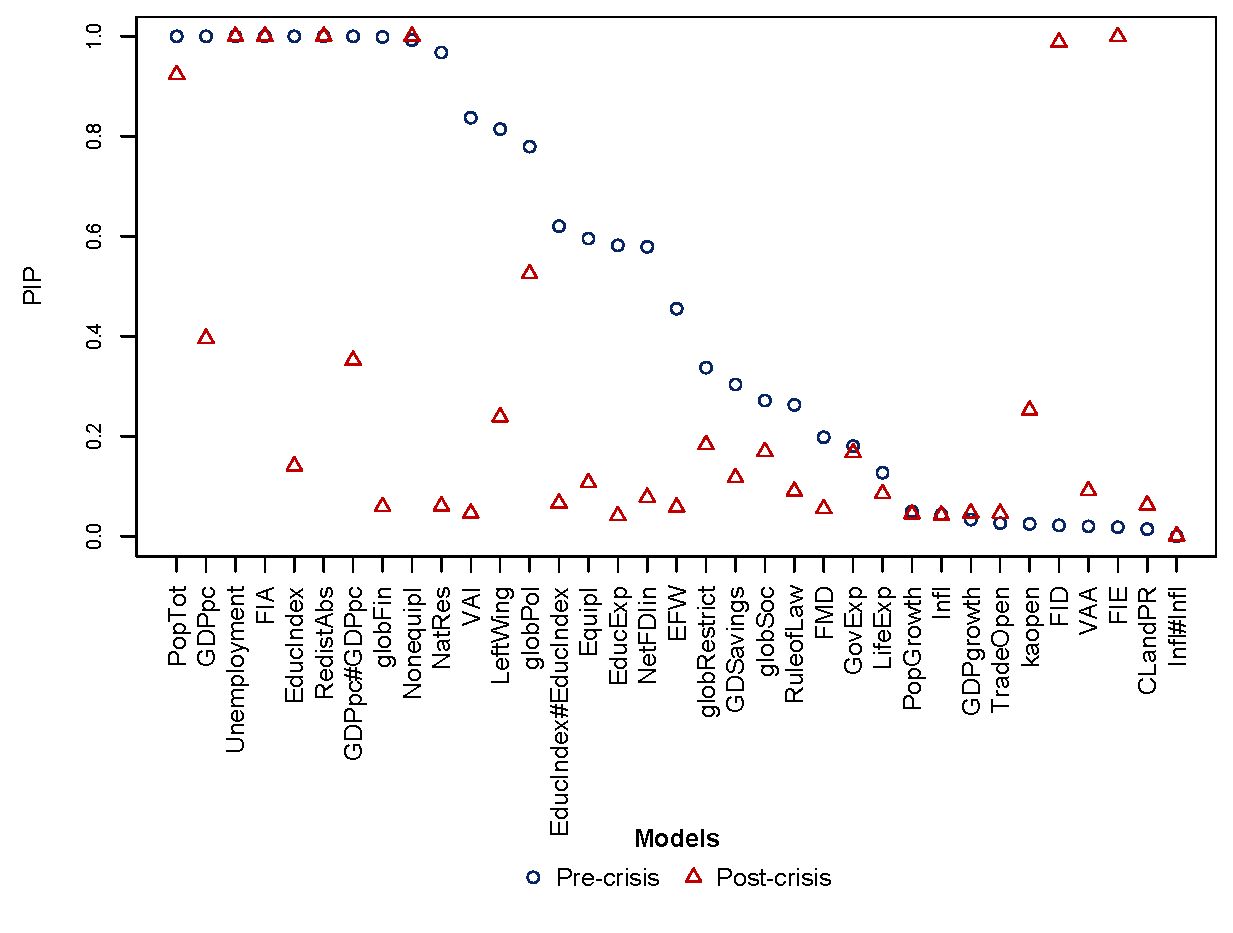
\includegraphics[width=0.8\textwidth, keepaspectratio]{Figures/ch4/comp_prepostcrisis_gini}
      % \begin{minipage}{0.8\textwidth}
        % \footnotesize
        % \emph{Note: The comparison only shows variables which show \ac{PIP} $> 0.9$ in at least one of the models.}
        % \end{minipage}
    \end{figure}

    \begin{figure}[ht!]
      \caption{Pre- / post- 2007 crisis comparison, top 10\% share}
      \label{ch4fig:comp_prepostcrisis_top10}
      \centering
      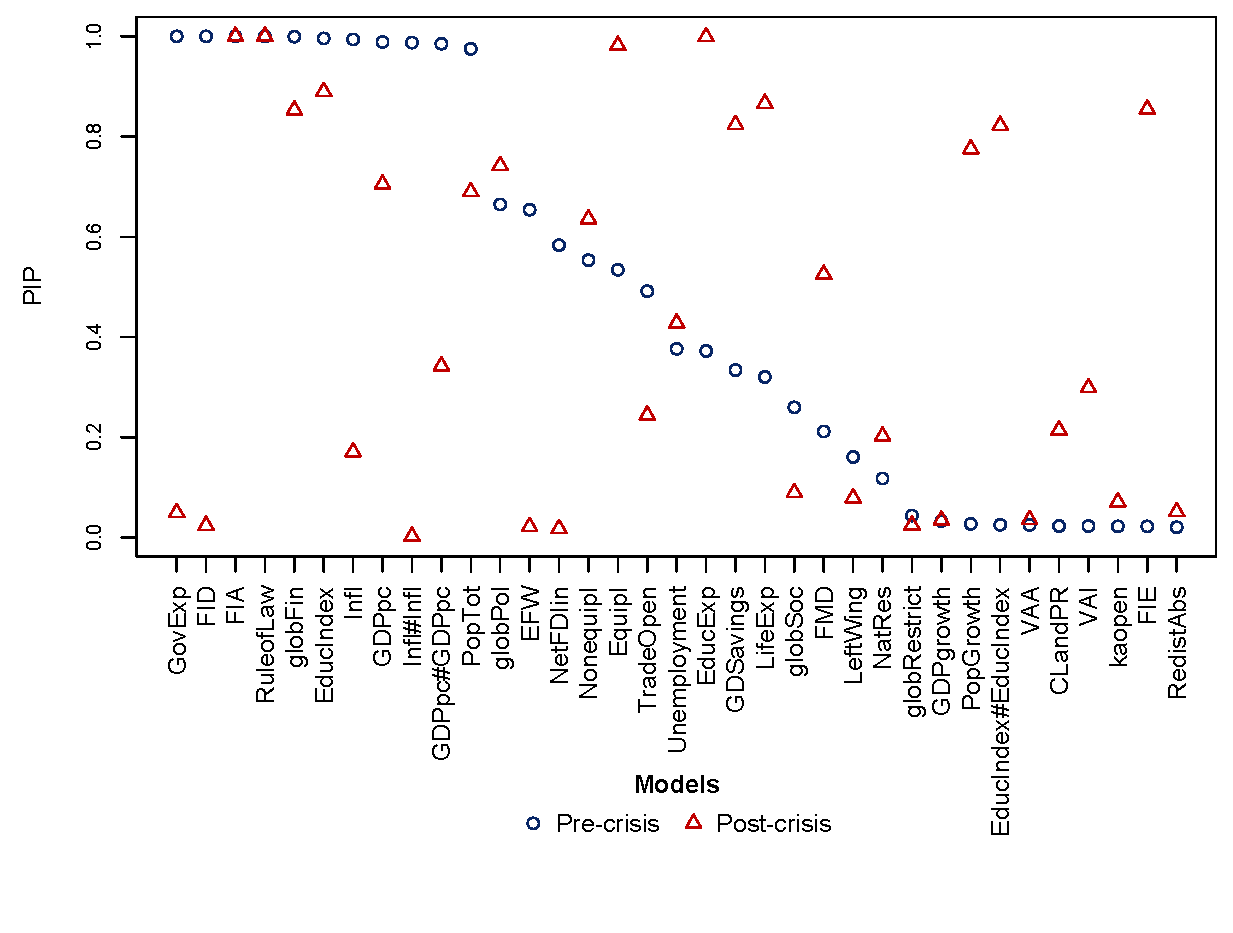
\includegraphics[width=0.8\textwidth, keepaspectratio]{Figures/ch4/comp_prepostcrisis_top10}
      % \begin{minipage}{0.8\textwidth}
        % \footnotesize
        % \emph{Note: The comparison only shows variables which show \ac{PIP} $> 0.9$ in at least one of the models.}
        % \end{minipage}
    \end{figure}

    \begin{figure}[ht!]
      \caption{Pre- / post- 2007 crisis comparison, top 1\% share}
      \label{ch4fig:comp_prepostcrisis_top1}
      \centering
      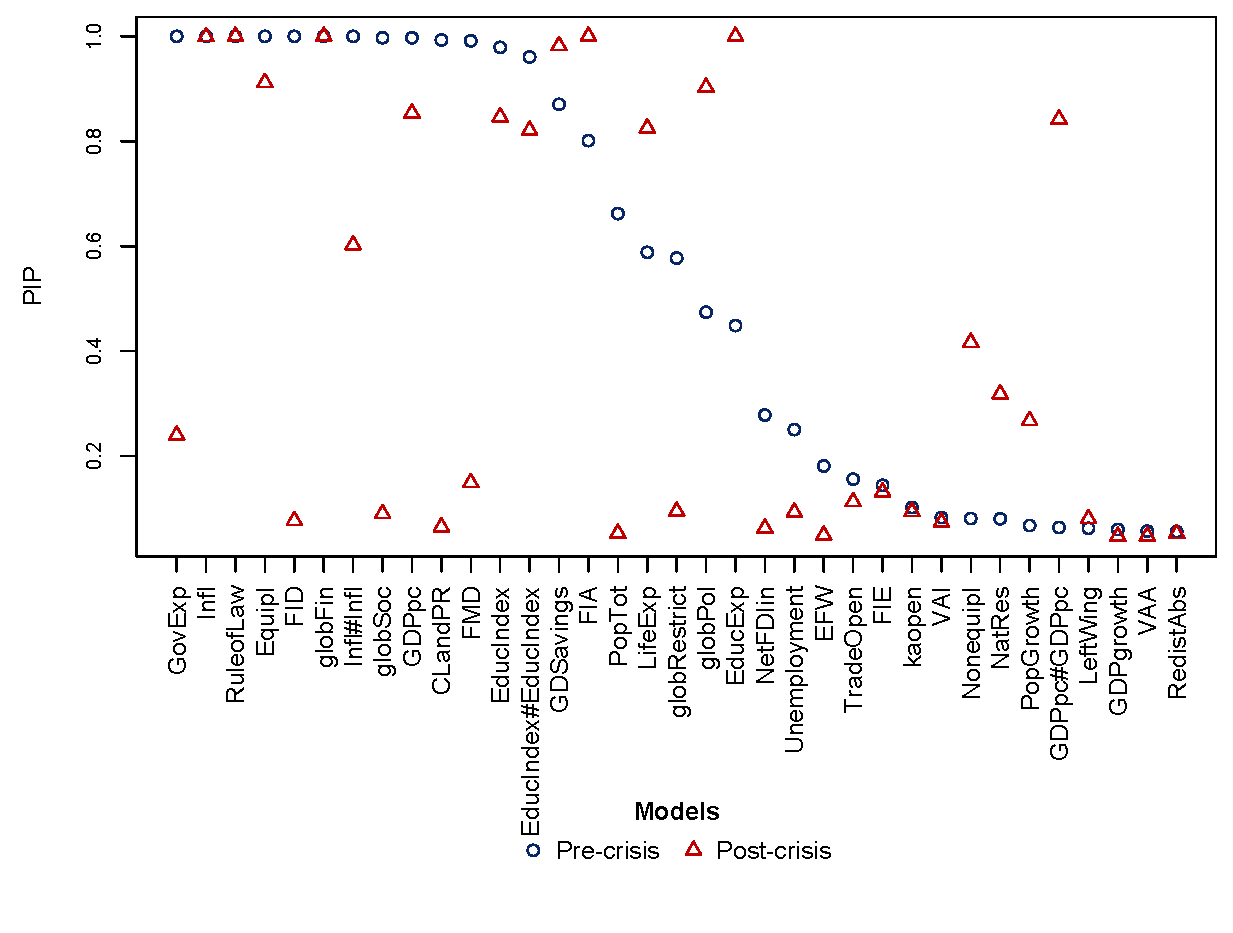
\includegraphics[width=0.8\textwidth, keepaspectratio]{Figures/ch4/comp_prepostcrisis_top1}
      % \begin{minipage}{0.8\textwidth}
        % \footnotesize
        % \emph{Note: The comparison only shows variables which show \ac{PIP} $> 0.9$ in at least one of the models.}
        % \end{minipage}
    \end{figure}

    \item \textit{Is endogeneity a potential problem here (similarly to the second paper) and how is it dealt with?}
    
    Based on similar arguments as in the second paper, endogeneity could be an issue. Moreover, financial indicators are not the only variables that could be potentially endogenous. Finding good instruments in the panel setting is, however, even more challenging than for the cross-section and Bayesian framework does offer directly applicable approaches such as system GMM, traditionally used in the literature. We limit the concerns here by relying on the lagged values of the explanatory variables in the estimation. This approach works well for the panel setting and largely confirms our findings from the baseline. Tables \ref{chA:tab4}, \ref{chA:tab5}, and \ref{chA:tab6} report the results for Gini index, top 10\%, and top 1\% share of income. I only report the variables with \ac{PIP} above 0.7. There are only minor changes in the inclusion probabilities of the top variables in case of income shares. More heterogeneity occurs with the estimation using the Gini index, where the effect of access and efficiency diminishes, but we see a substantial increase in the inclusion of FMD. This again warrants for caution in the interpretation of the latter set of results.

\end{enumerate}

\begin{table}[ht!]    
  \caption{Results using lagged explanatory variables, after-tax Gini index}\label{chA:tab4}
  \centering
  \footnotesize
  \begin{tabular}{lrrr}
    \toprule
  Variable & PIP & Post Mean & Post SD \\
    \midrule
    Education expenditures & 1.00 & -0.17932 & 0.06039 \\
    Value added in industry & 1.00 & -0.20504 & 0.06333 \\ 
    GDP per capita & 1.00 & 1.38484 & 0.66842 \\
    Education index (UN) & 1.00 & -0.52691 & 0.24553 \\ 
    Education index sq. & 1.00 & 0.68706 & 0.23271 \\
    Inflation & 1.00 & 0.36481 & 0.12373 \\
    Inflation sq. & 1.00 & -0.30380 & 0.11861 \\ 
    GDP per capita sq. & 1.00 & -1.70125 & 0.67566 \\ 
    Value added in agriculture & 1.00 & -0.16241 & 0.06386 \\ 
    Trade openness & 0.99 & 0.12535 & 0.05969 \\
    Restrictions on globalization & 0.98 & 0.16508 & 0.07073 \\
    Government expenditures & 0.93 & 0.10571 & 0.06467 \\ 
    Financial markets depth & 0.77 & 0.07140 & 0.06409 \\ 
    \bottomrule
  \end{tabular}
  \end{table}

  \begin{table}[ht!]    
    \caption{Results using lagged explanatory variables, top 10\% share}\label{chA:tab5}
    \centering
    \footnotesize
    \begin{tabular}{lrrr}
      \toprule
    Variable & PIP & Post Mean & Post SD \\
      \midrule
      Government expenditures & 1.00 & 0.22475 & 0.05339 \\
      GDP per capita & 1.00 & 2.20847 & 0.65929 \\
      Life expectancy & 1.00 & -0.57960 & 0.11207 \\ 
  Financial institutions depth & 1.00 & 0.21777 & 0.06570 \\
  Access to financial institutions & 1.00 & -0.23724 & 0.07999 \\
  Financial markets depth & 1.00 & 0.19877 & 0.05737 \\ 
  Education index (UN) & 1.00 & -0.67050 & 0.24141 \\
  GDP per capita\ sq. & 1.00 & -2.09554 & 0.67662 \\
  Education index\ sq. & 1.00 & 0.86813 & 0.22677 \\ 
  Financial globalization & 1.00 & -0.16380 & 0.06638 \\
  Left-wing orientation & 0.95 & 0.09576 & 0.05192 \\ 
  Trade openness & 0.88 & 0.10511 & 0.06732 \\
  Total population & 0.88 & 0.16140 & 0.10576 \\ 
  Net FDI (\% GDP) & 0.76 & -0.06376 & 0.05479 \\
  Equipment investment & 0.72 & -0.07970 & 0.07383 \\  
      \bottomrule
    \end{tabular}
    \end{table}

    \begin{table}[ht!]    
      \caption{Results using lagged explanatory variables, top 1\% share}\label{chA:tab6}
      \centering
      \footnotesize
      \begin{tabular}{lrrr}
        \toprule
      Variable & PIP & Post Mean & Post SD \\
        \midrule
        Government expenditures & 1.00 & 0.16178 & 0.05386 \\
        GDP per capita & 1.00 & 2.75765 & 0.66596 \\
        Life expectancy & 1.00 & -0.45941 & 0.09336 \\ 
        Access to financial institutions & 1.00 & -0.25288 & 0.07635 \\
        Financial markets depth & 1.00 & 0.15898 & 0.05719 \\ 
        Education index (UN) & 1.00 & -0.56127 & 0.22118 \\
        GDP per capita sq. & 1.00 & -2.64854 & 0.68373 \\ 
        Education index sq. & 1.00 & 0.73680 & 0.21445 \\
        Equipment investment & 1.00 & -0.16873 & 0.06436 \\ 
        Financial institutions depth & 1.00 & 0.15950 & 0.06642 \\
        Net FDI (\% GDP) & 0.96 & -0.09628 & 0.05042 \\ 
        Trade openness & 0.92 & 0.10741 & 0.06330 \\ 
        Financial globalization & 0.88 & -0.11499 & 0.07535 \\
        \bottomrule
      \end{tabular}
      \end{table}

\clearpage
\section{Prof. Dr. Ansgar H. Belke}
% {\itshape My comments on the above mentioned dissertation which is in the fields of research on financial development are as follows. 

% The idea behind this paper is nice, to take up-to date (Bayesian) econometric techniques and to apply them empirically to the issue of the relation between finance and growth and finance and inequality, respectively. The problem and topic of the individual papers, i.e. the chapters of the dissertation, is clearly set out in the abstract. And I also think – as will become obvious in the following – that the paper meets its own aims formulated in the introduction. 

% The dissertation deserves its main merits for its empirical efforts based on up-to-date econometric methods. The way in which the author implements his econometric strategies in the specific cases does appear overall adequate. 

% He has already published two papers contained in the dissertation in excellent refereed journals, i.e. the World Bank Economic Review and the Journal of International Money and Finance. These two papers form the first two chapters in the dissertation. He has written his third paper on the effect of financial development on income inequality by himself. It is very promising in terms of publication success as well. Most importantly, I can clearly recognize an original contribution of the author who has done all the excellent econometrics on his own.

% In his dissertation, the author proves his ability to grasp the main concepts, paraphrase them, and apply them. He is able to reflect on the main concept underlying the relevant theories and their interpretations. Seen on the whole, he proves to be intellectually independent. And there is sustained and direct engagement with the main research question. Hence, it does not come as a surprise that the author obviously widely understands the implications of his research questions and comes up with persuading answers to these research questions. 

% Concerning the structure of the argument it can be stated that the author has chosen a coherent and cogent structure which proceeds logically from point to point and paragraph to paragraph. There is a sustained train of thought throughout. Finally, it appears fair to say that the use of illustrating examples and tables and figures is judicious and highly appropriate. Moreover, there is a good balance between factual detail and key theoretical issues. 

% A large share of the relevant literature has been identified as well. The thesis is thus based on relevant references. 

% The thesis would also be defendable at my home institution or another respected institution where I gave lectures such as the Main University of Vienna (Austria) or the University of Hohenheim (Germany).

% In the following, I would like to deal with some minor issues which could be dealt with by the candidate in the upcoming defense:}

\begin{enumerate}
    \item \textit{A main issue to cope with in at least two of the papers (if not all) is endogeneity. The author should explain the strengths and weaknesses of the solutions found and applied in his papers to deal with this issue as, for instance, the use of lagged regressors etc. Are there some tasks and open issues left for future research in that respect?}
    
    In the first two chapters, we work with cross-sectional data in the estimations. There, we rely on several options to address endogeneity. The simplest approach uses the lagged values of the exogenous variables so that the potential for reverse effect is limited. As a second option, we apply 2SLS--BMA procedure and \ac{IVBMA}, and make use of instrumental variables. Our baseline findings are largely confirmed by the estimations that deal with endogeneity and we present the results in the respective chapters. In the fourth chapter's panel setting, we come back to using the lagged values of explanatory variables since finding good instruments in a panel is challenging and methods, such as system GMM not directly applicable in the Bayesian framework. Again, the results dominantly confirm the baseline findings. Nevertheless, especially the first chapter could be extended by updating the whole dataset and also making use of time variation in the data and using lagged values of explanatory variables. It could be a fruitful exercise in the near future as longer time spans of financial indicators will become available. 

    \item \textit{A linear functional form which is implicitly often assumed in the literature is fairly specific and, in some cases, even restrictive. It is important to distinguish specifications which can be examined in the framework of a linear regression from those which cannot. It is nice that the author thus checked for functional form beforehand and also implemented and estimated non-linear specifications. The author could comment a bit more on the chosen tests for non-linearity.}
    
    In general, we apply two approaches to capturing non-linearity. One lies in directly including the non-linear terms in the set of regressors. These are usually squared values of explanatory variables or interaction between variables, looking for a joint effect of, for example, institutions and financial development. The second approach is adjusting the sample and estimating the relationships in different periods (before and after crisis for in Chapter \ref{ch4}, before 1990 and after 1990 in Chapter \ref{ch2}), or for a different set of countries(high- vs. low- income in Chapter \ref{ch3}). We then compare the inclusion probabilities under these different settings. Due to the Bayesian nature of our estimation and in contrast to the frequentist approaches, we do not test for the differences in the alternative models (Chow test).

    \item \textit{What about (further) robustness checks? Does the author exploit all usual possibilities to conduct robustness checks (changes of the lag structure, explicit parameter restriction tests, preliminary sample split tests according to different policy regimes also beyond the financial crisis, changes of the criteria which serve as the basis for selecting the final presented empirical models such as information criteria) in the framework of his analysis? If not, please complement or at least be more explicit on what has been done.}

    I have extensively checked for robustness under varying priors, which is the key factor in the Bayesian analysis. I have also explored possible non-linearities (answer the previous comment notes some of the robustness checks to regimes switches). On top of that, I have put great effort into specifications that limit the endogeneity concerns. Although the set of potential checks often seems unbounded, I have looked thoroughly for both the methodologically critical and intellectually informative.

    \item \textit{At certain stages of his dissertation, the author applies cross-sectional data analysis. The author should be explicit about why he is not using panel data at these stages of analysis and what the trade-offs and sacrifices of this way of proceeding are.}
    
    We use the cross-sections mostly due to the limitations and unavailability of relevant data over time. This is the case of wealth inequality and for some financial development indicators. In the case of Chapter \ref{ch2} on finance and growth, the unavailability reason applies combined with the desire to have the results directly comparable to the previous studies by \textcite{Fernandezetal2001} and \textcite{SalaiMartin1997}. On the one hand, cross-sectional data allows us to make relatively general conclusions about the estimated relationship (in comparison with individual country studies based on time-series analysis), but at the same time, we abstract from any time variation of the data. This might not be big wrongdoing in terms of wealth inequality, which does not systematically change much in the short run. With some qualifications, we can also make a similar case for the long-run economic growth. However, we extend the analysis to panel data when possible in Chapter \ref{ch4} to strengthen our analysis, especially with the substantially larger number of data points for the estimation.

    \item \textit{So, is there any relevance of the paper for policy issues beyond that briefly and partly implicitly mentioned in the conclusions? I would appreciate if the authors would not only come up with testable hypotheses and the respective empirical results using readily available data but bring the very useful discussion of why and how finance matters for growth and inequality closer to the realm that is applicable to policymakers.}
    
    Thank you for pointing this out. I have included extended general policy implications discussed in the summary chapter of the dissertation.

    \item \textit{However, the summary of the dissertation is missing which should have given an overview of the dissertation and the research questions tackled therein. In this sense, it would have been quite useful as a guide for the reader.}
    
    I have amended the dissertation's summary, where I also elaborate on the policy implications of the thesis findings.

\end{enumerate}

\section{Martin \v{C}ih\'{a}k Ph.D.}

\textbf{a) Contribution}
\textit{Combined, the essays compiled in this thesis offer useful and original contributions to the considerable and expanding empirical literature on the intersection of finance, growth, and inequality. On a personal note, I have appreciated the ingenious use of the GFDD database that I spearheaded when I was at the World Bank. I find that this type of rigorous empirical approach can truly improve our understanding of the role of finance in the economy.}

\textit{I have three comments/suggestions for clarifications on the thesis\' contribution:}

\begin{enumerate}
    \item \textit{The document unfortunately appears to be incomplete, because Chapter 1 is missing/blank. The thesis would benefit from a well-crafted introductory chapter.}
    
    Thank you. Indeed, I have thoroughly amended the summary chapter of the dissertation.

    \item \textit{Given that chapters 2 and 3 are both joint with two coauthors (Mr. Mares being listed as the last of the three), it may be useful to clarify Mr. Mares's contribution. I presume that Mr. Mares has contributed significantly, but there is no way for me to ascertain the precise extent of Mr. Mares's involvement. It would be helpful for the thesis to contain an upfront disclosure/statement about the nature and scope of Mr. Mares's contribution to each of the co-authored essays (perhaps on the same page as the ``declaration of authorship''), indicating what are the contributions of Mr. Mares, and what are those of his coauthors.}
    
    Thank you for pointing this out. I comment on my contribution in the introductory chapter of the dissertation. My contribution is well appraised in the supervisor's report.

    \item \textit{Chapter 4 seems an extension of chapter 3, using the same Bayesian Model Averaging (BMA) approach to the finance-inequality nexus, the difference being that chapter 4 looks at income instead of wealth proxies. If there are other notable differences or contributions, it may be useful to flag any novel contributions upfront (perhaps in the forthcoming chapter 1).}
    
    Well taken point and similar to Mr. Ger\v{s}l's observation. I have adjusted the part on the value-added of the paper. I make four different points: 1) we efficiently account for model uncertainty as with the previous papers, 2) we use the \ac{WID} data on the top income shares, 3) we simultaneously consider different proxies of financial development to identify the most important ones, and 4) we do not merely examine multiple measures of income inequality for robustness checks, but we can to some extent distinguish diverse effects across the income distribution. I have reflected this also in the summary chapter of the dissertation.

\end{enumerate}

% \textbf{b) References}

% I have found the papers to be well-researched and generally well-motivated by gaps in the existing empirical literature. I provide some suggestions for references below.

% The thesis is relatively parsimonious, perhaps to the point of being telegraphic, on the theoretical front. The author concentrates on taking the empirical technique—BMA—to the data on finance and inequality. I do have sympathy for this heavily empirical approach. Nonetheless, for better balance, some more theoretical/conceptual discussion on the finance-inequality nexus would be useful.
% One of the key issues in the financial sector of the last decade has been the rise of shadow banking, and more recently the ascent of ``FinTech''. The thesis is focusing on banks, and for good reason. Nonetheless, it could come across as out-of-touch with the above developments, so I suggest to at least mention the rise of fintech and its potential effects, including on inequality.
% The thesis includes many relevant references, but the list is far from comprehensive, so perhaps that can be flagged upfront. Also, as part of strengthening the policy discussion, the author could reference the following relevant IMF Staff Discussion Notes (SDN):

% \begin{itemize}
% \item \href{https://www.imf.org/en/Publications/Staff-Discussion-Notes/Issues/2020/01/16/Finance-and-Inequality-45129}{SDN 20/01 ``Finance and Inequality''}
% \item \href{https://www.imf.org/en/Publications/Staff-Discussion-Notes/Issues/2018/09/17/women-in-finance-a-case-for-closing-gaps-45136}{SDN 18/05 ``Women in Finance: A Case for Closing Gaps''}
% \item \href{https://www.imf.org/en/Publications/Staff-Discussion-Notes/Issues/2016/12/31/Financial-Inclusion-Can-it-Meet-Multiple-Macroeconomic-Goals-43163}{SDN 15/17 ``Financial Inclusion: Can it Meet Multiple Macroeconomic Goals?''}
% \item \href{https://www.imf.org/en/Publications/Staff-Discussion-Notes/Issues/2016/12/31/Rethinking-Financial-Deepening-Stability-and-Growth-in-Emerging-Markets-42868}{SDN 15/08 ``Rethinking Financial Deepening: Stability and Growth in Emerging Markets''}
% \end{itemize}

% \textbf{c) Suitability for defense}
% The thesis has many strong aspects that certainly make it defendable. However, at my home institution, the IMF, I would expect the study to include a clearer discussion of policy implications, and an overall summary. In that context, it is a pity that chapter 1 (``Summary of the dissertation'') is blank in the current draft. For the next/revised draft, I would suggest including chapter 1, which should ideally pull together the various storylines from the three separate essays and weave them into one coherent whole.

% \textbf{d) Suitability for publication}

% There is no doubt in my mind that much of the thesis is publishable in respected journals. I have enjoyed reading the essays, especially chapters 2 and 3.
% Chapter 1 is missing, so it is hard to pass judgement, but chapter 2 has already been published in the World Bank Economic Review. Moreover, chapter 3—already issued as an IES working paper—is forthcoming in Journal of International Money and Finance, so it is certainly publishable. Chapter 4 appears relatively less ripe than the other two essays, but even that chapter can be suitable for publication. With chapter 4, readers may wonder about its contribution relative to chapter 3. Both chapters feature a heavy use of Bayesian Model Averaging (BMA) to study the link between finance and inequality. A difference is that chapter 3 focuses on wealth proxies while chapter 4 looks as income proxies, but some readers may be left wondering about the relative value added of chapter 4 and whether the two could perhaps be combined.

\textbf{e) Comments}
\begin{enumerate}
    \item \textit{In chapter 2, the finding that quality of finance matters is intellectually appealing, but I would caution that the measure of net interest margin is only a partial proxy for ``efficiency''. In particular, net interest margin captures factors such as asset composition of financial intermediaries. To truly evaluate efficiency of financial intermediaries, one needs to look also at other measures, such as cost-to-income ratios or overhead costs to total assets (which are also in the GFDD). Following up on the earlier general point, having a solid conceptual/theoretical discussion of ``efficiency of financial intermediaries'' may be helpful before diving into the BMA and using it on the net interest margin as a proxy.}
    
    Thank you for the suggestion. I agree that the careful definition of what we understand behind the efficiency of financial institutions is critical for the discussion throughout the dissertation chapters. We may have used it too heedlessly in the paper on finance-growth nexus. I used the summary chapter to shed some light upon this issue and included a part where I attempt to conceptualize what we refer to as efficiency of finance and stress the limitations presented by the use of proxies. We use the other indicators (overhead costs, return on assets/equity) in the later papers. The choice of net interest margin in the first paper was dictated dominantly by the country-coverage at the time of writing.
    
    \item \textit{In chapter 2, the discussion on nonlinearity (section 2.5.3) comes across as an afterthought. Given the massive attention in the recent literature on nonlinearities in the relationship between finance and growth, it is surprising to see this aspect to receive only a relatively scant attention. Nonlinearity in the finance-growth nexus (and finance-inequality nexus) may well be a part of the reason why linear relationships (examined in much of this paper) can come out insignificant.}
    
    I understand the concern, but we note the non-linearity already in the paper's introduction and thoroughly examine it later in the devoted section (now \ref{ch2subsec:nonlin}). We do not find relevance for the non-linear terms, either quadratic transformations or interactions between the financial development indicators, under any scenario. This is why we also present the results as a robustness check rather than as a baseline for the paper.

    \item \textit{In chapters 3 and 4, it would be helpful to clarify the different concepts of inequality, how they are measured, and how they relate to each other. It is important to flag that the precision of some commonly used inequality indicators has become a subject of major public controversy and discussion (Auten and Splinter 2019; Bhalla 2017; Economist 2019) In light of these important debates, a fuller discussion of weaknesses of existing inequality measures seams important. Please consider adding (and discussing) the following references:}
     \begin{itemize}
        \item Auten, Gerald, and David Splinter. 2019. ``Top 1 Percent Income Shares: Comparing Estimates Using Tax Data.'' AEA Papers and Proceedings 109:307–11.
        \item Bhalla, Surjit S. 2017. The New Wealth of Nations. Simon and Schuster
        \item Economist. 2019. ``Inequality Illusions: Why Wealth and Income Gaps Are Not What They Appear.'' November 30
      \end{itemize}
    
      Thank you for directing me towards additional resources. I am aware of the current contests about inequality measurement in the literature. I have devoted part of the summary chapter to measurement issues, including discussion of selected references. In setting up the right policies to address inequality trends, I believe the issue is fundamental. At the same time, as long as the measurement issues are not dramatically heterogeneous across countries and time (which we, unfortunately, cannot completely rule out), consistently collected and constructed data may inform us on the causes and consequences of inequality irrespective of the precise numbers put on various measures of inequality. Lastly, the discussion on the wealth/income inequality differences is part of Chapter \ref{ch3}, and I cover the measurement of inequality measures employed in the respective chapters. 

    \item \textit{Chapter 3: given the importance of instruments for the BMA estimation, please consider a more specific discussion of the instruments. For example, why is the average of areas 3D, 4C, 4D, and 5A of the EFW a suitable instrument? The authors claim that ''components of our financial liberalization measure are exogenous to the wealth inequality as the change in wealth distribution is improbably to have direct effect on any of them``. It is unclear where this assertion comes from, so if there is evidence for it, I suggest adding it. There is some evidence to the contrary, at least for income inequality (see for example Sylwester, Kevin, 2010, Journal of Applied Economics), finding strong evidence of links between inequality and the black market premium (which is one of the EFW areas, namely 4C).}
    
    The instrumental variable approach relies heavily on good instrument choice, and their qualification may almost universally be disputed \parencite{deaton2010instruments}. Nevertheless, we found the genetic distance and selected components of EFW (also used as financial liberalization proxy by \textcite{de2017finance}), to be reasonable instruments empirically and conceptually. I have read \textcite{sylwester2003changes} with interest. He associates the black market premium with income inequality, but the focus is on the link from black market premium to inequality rather than the other way around. Moreover, he is not definite on the mechanism through which the association works and as one of the promising routes, he marks interest rate differential (from LIBOR). Such a mechanism, in fact, largely supports our choice of black-market premium as an instrument for financial development indicators, provided that the effect goes \emph{only} through financial channels. 
        
    \item \textit{Chapter 4 departs from much of existing literature by considering the after-tax rather than the before-tax income distribution as a dependent variable. However, the rationale for this choice is not well explained. In fact, one could make the case for considering before-tax income distribution, because that's the one where financial sector's role is likely to be more prominent/visible (and more separable from the effects of other policies, including fiscal).}
    
    I agree with the practical note. We rely on the after-tax income Gini coefficient as we also include the redistribution variable among the regressors to indirectly account for taxation and transfers, as coverage of exact data on the two is scarce. Since we define it as a difference between before-tax and after-tax Gini coefficients, the estimate is not substantially influenced by using either of the two as the dependent variable. The switch changes only the sign of the posterior mean of redistribution. This supports the point by \textcite{furceri2019robust} that unless redistribution is systematically correlated with other regressors, their effect on the net and gross inequality should be the same. In our case, using after-tax allows for more intuitive interpretation. I address this issue also in the earlier response above. Please refer to Table \ref{chA:tab3}, where I provide the estimation with the before-tax Gini coefficient as the dependent variable. I report only the regressors with \ac{PIP} above 0.7 as the results are nearly identical to the baseline estimate. 

    \item \textit{The thesis --- across the chapters --- would benefit from strengthening the discussion on policy implications. For example, chapter 2 says that ``the current wave of regulatory changes intended to safeguard financial stability should carefully analyze the consequences for the efficiency of financial intermediaries,'' which would benefit from clarification. Are the authors suggesting to reorient micro- and macro-prudential supervisors from safeguarding financial stability to targeting efficiency of financial intermediaries? (I presume not, but the text could be misread that way.) Also, the reference to ``the current wave of regulatory changes'' seems outdated and misleading, given that the post-crisis regulatory wave has already taken place (and we are now in the stage where some countries are considering regulatory roll-backs.)}
    
    This point is well taken. I have reworded part of the policy conclusions included and extended the discussion on overall policy implications in the summary chapter of the dissertation.

    \item \textit{Chapter 2, page 20: the regression includes various dummy variables, such as the one for Sub-Saharan Africa and the ``fraction of Confucian population'' (which is close to a proxy for China). Given the importance of these regions, I worry that the estimated coefficients on those dummy variables are just proxies for our ignorance about the underlying drivers of the finance-growth relationship. It would be useful to include a solid discussion on these dummy variables.}
    
    Your concern is valid. Sub-Saharan Africa and Latin America dummie, along with a fraction of the Confucian population, may distort not only the effect of financial variables, but perhaps further regressors. Sub-Sahara dummy also shows a high correlation with other variables. It is one of the reasons we dropped it in the second paper on finance and wealth inequality. Note that the effect of Sub-Saharan countries diminishes when we consider other financial indicators additionally to private credit, so this could be some evidence it is masking effects related to financial development (although in a shorter period of 2000's its \ac{PIP} jumps up again, perhaps driven by specific time period assumed). The fraction of the Confucian population likely captures the extraordinary growth rate of particular countries for the large part of the period we explore, but China is not among them as it is not present in our sample. The countries with the highest fraction of the Confucian population are South Korea, Hong Kong, and Singapore. Hopefully, as the data collection progresses, future research will be able to fully abstract from these variables. 

    \item \textit{Chapter 2, front page footnote: ``the The World Bank Econonmic Review'' should read ``The World Bank Economic Review''.}
    
    Corrected. Thank you for pointing it out.
\end{enumerate}

\clearpage
\printbibliography[heading=subbibliography]
\addcontentsline{toc}{section}{References}